% Exact bipartite comparison on six vertices: 2*4=8 versus 3*3=9.
% All possible cross-group edges are shown; no intra-group edges.
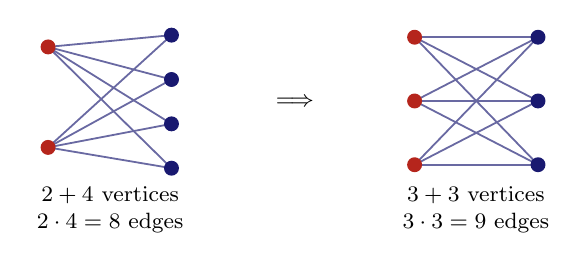
\begin{tikzpicture}[x=0.95cm,y=0.88cm,line cap=round]
  \foreach \a in {0,1}{
    \foreach \b in {0,1,2,3}{
      \draw[MidnightBlue!65,line width=0.65pt] (0.7,{0.45+1.45*\a}) -- (2.35,{0.15+0.64*\b});
    }
  }
  \foreach \a in {0,1}{
    \fill[BrickRed] (0.7,{0.45+1.45*\a}) circle (2.7pt);
  }
  \foreach \b in {0,1,2,3}{
    \fill[MidnightBlue] (2.35,{0.15+0.64*\b}) circle (2.7pt);
  }
  \foreach \a in {0,1,2}{
    \foreach \b in {0,1,2}{
      \draw[MidnightBlue!65,line width=0.65pt] (5.6,{0.2+0.92*\a}) -- (7.25,{0.2+0.92*\b});
    }
  }
  \foreach \a in {0,1,2}{
    \fill[BrickRed] (5.6,{0.2+0.92*\a}) circle (2.7pt);
    \fill[MidnightBlue] (7.25,{0.2+0.92*\a}) circle (2.7pt);
  }
  \node[font=\footnotesize,align=center] at (1.53,-0.45) {$2+4$ vertices\\$2\cdot4=8$ edges};
  \node[font=\footnotesize,align=center] at (6.42,-0.45) {$3+3$ vertices\\$3\cdot3=9$ edges};
  \node[font=\footnotesize] at (4.0,1.1) {$\Longrightarrow$};
\end{tikzpicture}
